\chapter{مقدمه}

در سال‌های اخیر، توسعه سریع فناوری‌های مبتنی بر داده و نیاز روزافزون به تحلیل هوشمند اطلاعات، موجب رشد چشم‌گیر الگوریتم‌های یادگیری ماشین و یادگیری عمیق شده است. در این میان، مدل‌های مبتنی بر معماری‌های شبکه‌های عصبی، به‌ویژه در حوزه‌هایی چون پردازش زبان طبیعی، بینایی ماشین، و تحلیل سری‌های زمانی، جایگاه ویژه‌ای یافته‌اند. یکی از تحولات بنیادی در این مسیر، ظهور معماری مبدل ها \footnote{\lr{Transformer}} بوده است که با بهره‌گیری از مکانیزم توجه، رویکردی نوین و موثر برای مدل‌سازی وابستگی‌های طولانی در داده‌های ترتیبی ارائه می‌دهد. درک جایگاه و کارکرد این معماری، مستلزم شناخت دقیق‌تر از مفاهیم بنیادین در هوش مصنوعی، یادگیری ماشین، شبکه‌های عصبی و ساختارهای بازگشتی است. از این‌رو، فصل حاضر به‌منظور ارائه بستر نظری لازم، به بررسی سیر تاریخی هوش مصنوعی، معرفی روش‌های یادگیری ماشین، مروری بر الگوریتم‌های کلاسیک، و تحلیل ساختار شبکه‌های بازگشتی از جمله شبکه های حافظه کوتاه مدت طولانی \footnote{\lr{LSTM}} اختصاص دارد.




\subsection{آغاز هوش مصنوعی و هدف اصلی}

هوش مصنوعی به عنوان شاخه‌ای از علوم کامپیوتر، در دهه ۱۹۵۰ با هدف ساخت سیستم‌ها و ماشین‌هایی که توانایی تقلید از هوش انسانی را دارند، آغاز شد. نخستین بار، مکارتی \footnote{\lr{John McCarthy}} در سال ۱۹۵۶ این اصطلاح را به کار گرفت \cite{mccarthy1956proposal} و هوش مصنوعی به عنوان علمی که در آن به مطالعه الگوریتم‌هایی برای تقلید رفتار انسانی می‌پردازد، شناخته شد. اهداف اولیه هوش مصنوعی شامل توانایی درک زبان، یادگیری، حل مسئله و تولید موجودات هوشمند بود. در این دوران پروژه‌های تحقیقاتی زیادی به امید دستیابی به هوش مصنوعی عمومی \footnote{\lr{AGI, Artificial General Intelligence}}
شروع به کار کردند \cite{crevier1993ai,nilsson2010quest}.

\subsection{دورهٔ طلایی و پیشرفت‌های اولیه}

در دهه ۵۰ و ۶۰ میلادی، هوش مصنوعی\footnote{\lr{Artificial Intelligence (AI)}} به عنوان یکی از پرچمداران پژوهش‌های نوین شناخته می‌شد. الگوریتم‌های اولیه با تکیه بر روش‌های منطقی و ریاضیاتی برای حل مسئله و بازی‌های ساده توسعه یافتند؛ مانند انواع الگوریتم‌های جستجوی درختی\footnote{\lr{Tree Search Algorithms}} که در این دوره به وجود آمدند و زمینه‌ساز اولین دستاوردهای هوش مصنوعی در بازی‌های تخته‌ای\footnote{\lr{Board Games}} همچون شطرنج\footnote{\lr{Chess}} شدند \cite{newell1959report}. 

در این دوران، پیشرفت‌های بیشتری در پردازش زبان طبیعی\footnote{\lr{Natural Language Processing (NLP)}} و سیستم‌های خبره\footnote{\lr{Expert Systems}} نیز صورت گرفت که این امید را در دانشمندان و محققان تقویت کرد که دستیابی به هوش مصنوعی عمومی\footnote{\lr{Artificial General Intelligence (AGI)}} به‌زودی ممکن خواهد بود \cite{feigenbaum1983handbook}.


\subsection{انتظارات بیش از حد و ظهور عصر تاریک}

با وجود پیشرفت‌های هوش مصنوعی، محدودیت‌های تکنولوژی (مثل عدم وجود  پردازنده های گرافیکی  \footnote{\lr{GPU}} پرقدرت در آن زمان) و همچنین کمبود داده‌های کافی برای آموزش مدل‌های پیچیده‌تر، باعث شد که بسیاری از پروژه‌های تحقیقاتی نتوانند به نتایج پیش‌بینی‌شده قابل قبول دست یابند. در نتیجه، هوش مصنوعی در دهه ۷۰ به مرحله‌ای از رکود وارد شد که به آن عصر تاریک هوش مصنوعی یا زمستان هوش مصنوعی \footnote{\lr{AI Winter}} می‌گویند \cite{lighthill1973artificial,crevier1993ai}. در این دوران، بسیاری از پروژه‌ها تعطیل و سرمایه‌گذاری‌ها قطع شدند و دولت‌ها و سازمان‌های سرمایه‌گذار به دلیل عدم دستیابی به نتایج مطلوب از ادامه سرمایه‌گذاری منصرف شدند.


\subsection{عوامل اصلی عصر تاریک هوش مصنوعی}


\textbf{محدودیت‌های سخت‌افزاری:} در آن زمان، سیستم‌های اولیه هوش مصنوعی به محاسبات سنگینی نیاز داشتند که با توان پردازشی محدود آن دوره همخوانی نداشت \cite{nilsson2010quest}.

\textbf{کمبود داده‌ها:} در آن زمان، دسترسی به داده‌های کافی برای آموزش مدل‌های پیچیده ممکن نبود و الگوریتم‌های موجود به داده‌های بیشتری نیاز داشتند تا بتوانند به‌درستی آموزش ببینند و عملکرد مطلوبی داشته باشند \cite{crevier1993ai}.

\textbf{روش‌های محدود یادگیری:} الگوریتم‌های اولیه به شدت به برنامه‌ریزی انسانی وابسته بودند و در بسیاری از موارد، مدل‌ها قادر به تعمیم به مسائل جدید نبودند و نمی‌توانستند تعمیم‌پذیری خیلی بالایی داشته باشند \cite{russell2016artificial}.



\subsection{پایان عصر تاریک و بازگشت هوش مصنوعی}

پس از چندین سال رکود و عدم سرمایه‌گذاری در حوزهٔ هوش مصنوعی، سرانجام در دهه ۱۹۸۰ و ۱۹۹۰ عصر تاریک هوش مصنوعی با تحولات تکنولوژی و از همه مهم‌تر ظهور سیستم‌های خبره به پایان رسید \cite{feigenbaum1983handbook}. سیستم‌های خبره به عنوان یکی از اولین تلاش‌های موفق برای کاربردهای صنعتی در هوش مصنوعی به‌وجود آمدند. بر خلاف الگوریتم‌های اولیه، این سیستم‌ها از پایگاه بزرگ قواعد و قوانین \footnote{\lr{\lr{Rule Based Systems}}} استفاده می‌کردند. در سیستم‌های خبره، به جای تلاش برای شبیه‌سازی کلی هوش مصنوعی، بر حل مسائل تخصصی برای صنایع و سازمان‌ها تمرکز می‌شد. برای مثال، سیستم‌های خبره در پزشکی برای تشخیص بیماری‌ها و پیشنهاد درمان، در صنعت برای مدیریت و پیش‌بینی خرابی ماشین‌آلات، و در امور مالی برای تحلیل و ارزیابی ریسک کاربرد داشتند \cite{mccorduck2004machines}.

هرچند این سیستم‌ها نمی‌توانستند درک عمیق و هوشمندی عمومی را ایجاد کنند، اما برای رفع نیازهای پیچیده مناسب بودند. همزمان با موفقیت این سیستم‌ها، بهبودهای زیادی در سخت‌افزارها و کاهش هزینه‌های پردازش به وجود آمد. در دهه‌های ۱۹۸۰ و ۱۹۹۰، کامپیوترها به تدریج قوی‌تر و مقرون به صرفه‌تر شدند و امکان پردازش داده‌های بیشتر و اجرای الگوریتم‌های پیچیده‌تر فراهم شد. این افزایش توان محاسباتی، نیاز به پردازش داده‌های بزرگ و پیچیده را برآورده کرد و در نتیجه دسترسی به داده‌ها و انجام محاسبات سنگین برای توسعه الگوریتم‌های جدید تسهیل شد. از سوی دیگر، پیشرفت‌های انجام‌شده در ذخیره‌سازی داده و رشد اینترنت باعث دسترسی گسترده‌تر به داده‌ها و منابع اطلاعاتی گردید \cite{nilsson2010quest}.

به این ترتیب، مجموعه‌ای از عوامل، شامل ظهور سیستم‌های خبره، افزایش قدرت پردازش و دسترسی به داده‌های بیشتر، منجر به بازگشت هوش مصنوعی شد. این دوره نه تنها پایان عصر تاریک هوش مصنوعی بود، بلکه راه را برای الگوریتم‌های یادگیری ماشین و توسعهٔ شبکه‌های عصبی هموار کرد \cite{russell2016artificial}.


\section{انواع مدل یادگیری ماشین و شبکه‌های عصبی}\label{sec:ml-types}
یادگیری ماشین و شبکه‌های عصبی به عنوان دو زیرشاخه مهم از هوش مصنوعی، در سال‌های اخیر به‌طور گسترده‌ای مورد توجه پژوهشگران و صنعت قرار گرفته‌اند. این مدل‌ها با هدف یادگیری الگوها و روابط موجود در داده‌ها توسعه یافته‌اند و امروزه در حوزه‌های مختلفی از جمله بینایی ماشین، پردازش زبان طبیعی، پیش‌بینی سری‌های زمانی و داده‌کاوی مورد استفاده قرار می‌گیرند \cite{bishop2006pattern,mitchell1997machine,murphy2012machine}.

\subsection{یادگیری ماشین: مروری کلی}
یادگیری ماشین \footnote{\lr{Machine Learning}} شاخه‌ای از هوش مصنوعی است که به مدل‌های محاسباتی این امکان را می‌دهد الگوها را از داده‌ها به شکل خودکار یاد بگیرند و بتوانند تصمیم‌گیری کنند
\cite{goodfellow2016deep,mitchell1997machine}.
در واقع، هدف یادگیری ماشین این است که مدل‌ها بتوانند از داده‌ها الگوها و روابط پنهان را استخراج کنند و به نتایج و تصمیم‌های قابل اعتماد دست یابند.

\subsection{تقسیم‌بندی‌های اصلی در یادگیری ماشین}
به طور کلی، یادگیری ماشین به سه دستهٔ اصلی تقسیم می‌شود:
\begin{itemize}
 	\item یادگیری با نظارت\footnote{\lr{Supervised Learning}}
	\item یادگیری بدون نظارت\footnote{\lr{Unsupervised Learning}}
	\item یادگیری تقویتی\footnote{\lr{Reinforcement Learning}}	
\end{itemize}
این طبقه‌بندی در بسیاری از کتاب‌ها و مراجع مهم یادگیری ماشین مطرح شده است
\cite{bishop2006pattern,murphy2012machine}.

\subsection{یادگیری نظارت‌شده}
یادگیری نظارت‌شده یکی از رایج‌ترین روش‌ها در یادگیری ماشین شناخته می‌شود که در آن از مجموعه داده‌های برچسب‌گذاری‌شده برای آموزش مدل استفاده می‌کنیم \cite{james2013introduction}. هدف این الگوریتم تشخیص الگوها در میان داده‌های ورودی است تا بتواند روی داده‌های جدید پیش‌بینی یا طبقه‌بندی انجام دهد. این نوع شامل دو دسته الگوریتم رگرسیون \footnote{\lr{Regression}} و کلاس بندی\footnote{\lr{Classification}} می‌شود.


\subsubsection{کلاس‌بندی}

در میان روش‌های یادگیری با نظارت، \textbf{کلاس‌بندی} \footnote{\lr{Classification}} یکی از پرکاربردترین مسائل محسوب می‌شود. هدف در این مسئله، تخصیص هر نمونه ورودی به یکی از برچسب‌های گسسته از پیش تعریف‌شده است. مدل با استفاده از داده‌های آموزشی که شامل ویژگی‌ها و برچسب صحیح هستند، الگوهای حاکم بر داده را می‌آموزد و تلاش می‌کند بر اساس آن، داده‌های جدید را به دسته مناسب اختصاص دهد. این روش در کاربردهای متنوعی نظیر تشخیص هرزنامه\footnote{\lr{Spam Detection}}، شناسایی بیماری‌ها، طبقه‌بندی تصاویر و تحلیل احساسات به‌طور گسترده مورد استفاده قرار می‌گیرد \cite{bishop2006pattern,murphy2012machine}.


\begin{figure}[h]
	\centering
	\begin{minipage}[b]{0.7\textwidth}
		\centering
		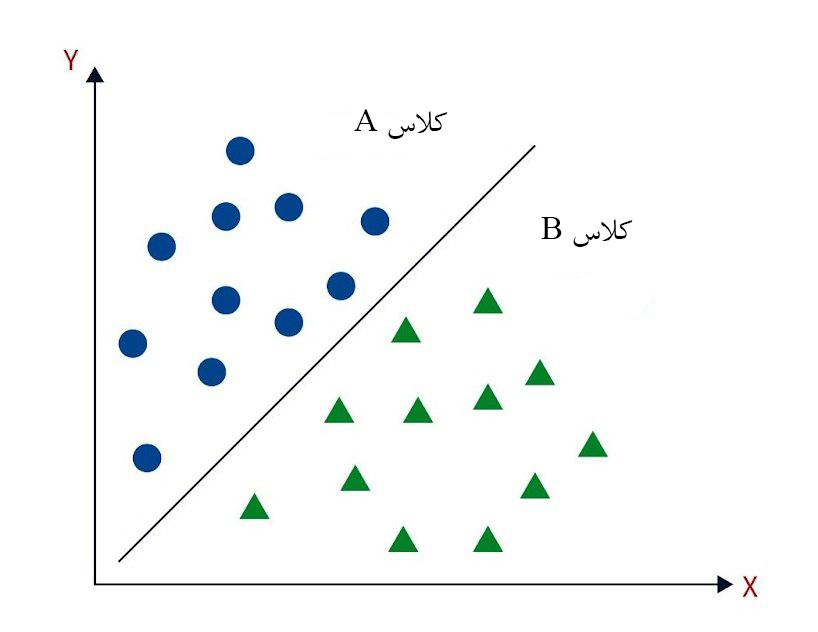
\includegraphics[width=\textwidth]{transformer_images/persian images/b15.png}
		\caption{کلاس بندی}
		\label{fig:classification}
	\end{minipage}
	\hfill
\end{figure}



\subsubsection{رگرسیون}

در مقابل، \textbf{رگرسیون} \footnote{\lr{Regression}}  به مسئله پیش‌ بینی مقادیر پیوسته می‌پردازد. در این نوع از یادگیری نظارت‌شده، مدل می‌کوشد رابطه‌ای میان متغیرهای ورودی و خروجی‌های عددی برقرار کند تا بر اساس آن، بتواند خروجی نمونه‌های جدید را تخمین بزند. تفاوت اصلی رگرسیون با کلاس‌بندی در ماهیت خروجی است؛ به‌طوری‌که در رگرسیون، خروجی به جای دسته‌بندی، یک مقدار عددی خواهد بود. از جمله کاربردهای رایج این نوع مدل‌ها می‌توان به پیش‌بینی قیمت مسکن، تخمین میزان فروش، و پیش‌بینی وضعیت آب‌وهوا اشاره کرد \cite{montgomery2021introduction}.


\begin{figure}[h]
	\centering
	\begin{minipage}[b]{0.7\textwidth}
		\centering
		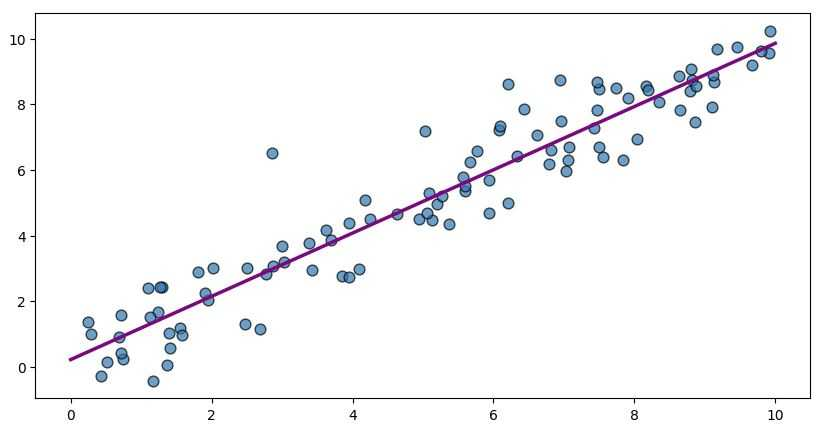
\includegraphics[width=\textwidth]{transformer_images/regression.jpg}
		\caption{رگرسیون}
		\label{fig:regerssion}
	\end{minipage}
	\hfill
\end{figure}



\subsection{یادگیری بدون نظارت}

یادگیری بدون نظارت \footnote{\lr{Unsupervised Learning}} نوعی از روش‌های یادگیری ماشین است که در آن مدل بدون استفاده از برچسب‌های خروجی، سعی در کشف الگوها، ساختارها یا روابط پنهان میان داده‌ها دارد \cite{bishop2006pattern}. در این رویکرد، داده‌های ورودی تنها شامل ویژگی‌ها هستند و هدف، گروه‌بندی یا استخراج ساختار درونی آن‌ها بدون دانش قبلی از دسته‌بندی صحیح است. برخلاف یادگیری با نظارت که مدل از پاسخ صحیح برای آموزش استفاده می‌کند، در یادگیری بدون نظارت، مدل باید به‌تنهایی ساختارهای معنادار را در داده‌ها کشف کند.

از کاربردهای رایج یادگیری بدون نظارت می‌توان به خوشه‌بندی \footnote{\lr{Clustering}}، کاهش ابعاد \footnote{\lr{Dimensionality Reduction}}، آشکارسازی ناهنجاری‌ها \footnote{\lr{Anomaly Detection}}، و استخراج ویژگی‌ها اشاره کرد. 



\begin{figure}[h]
	\centering
	\begin{minipage}[b]{0.7\textwidth}
		\centering
		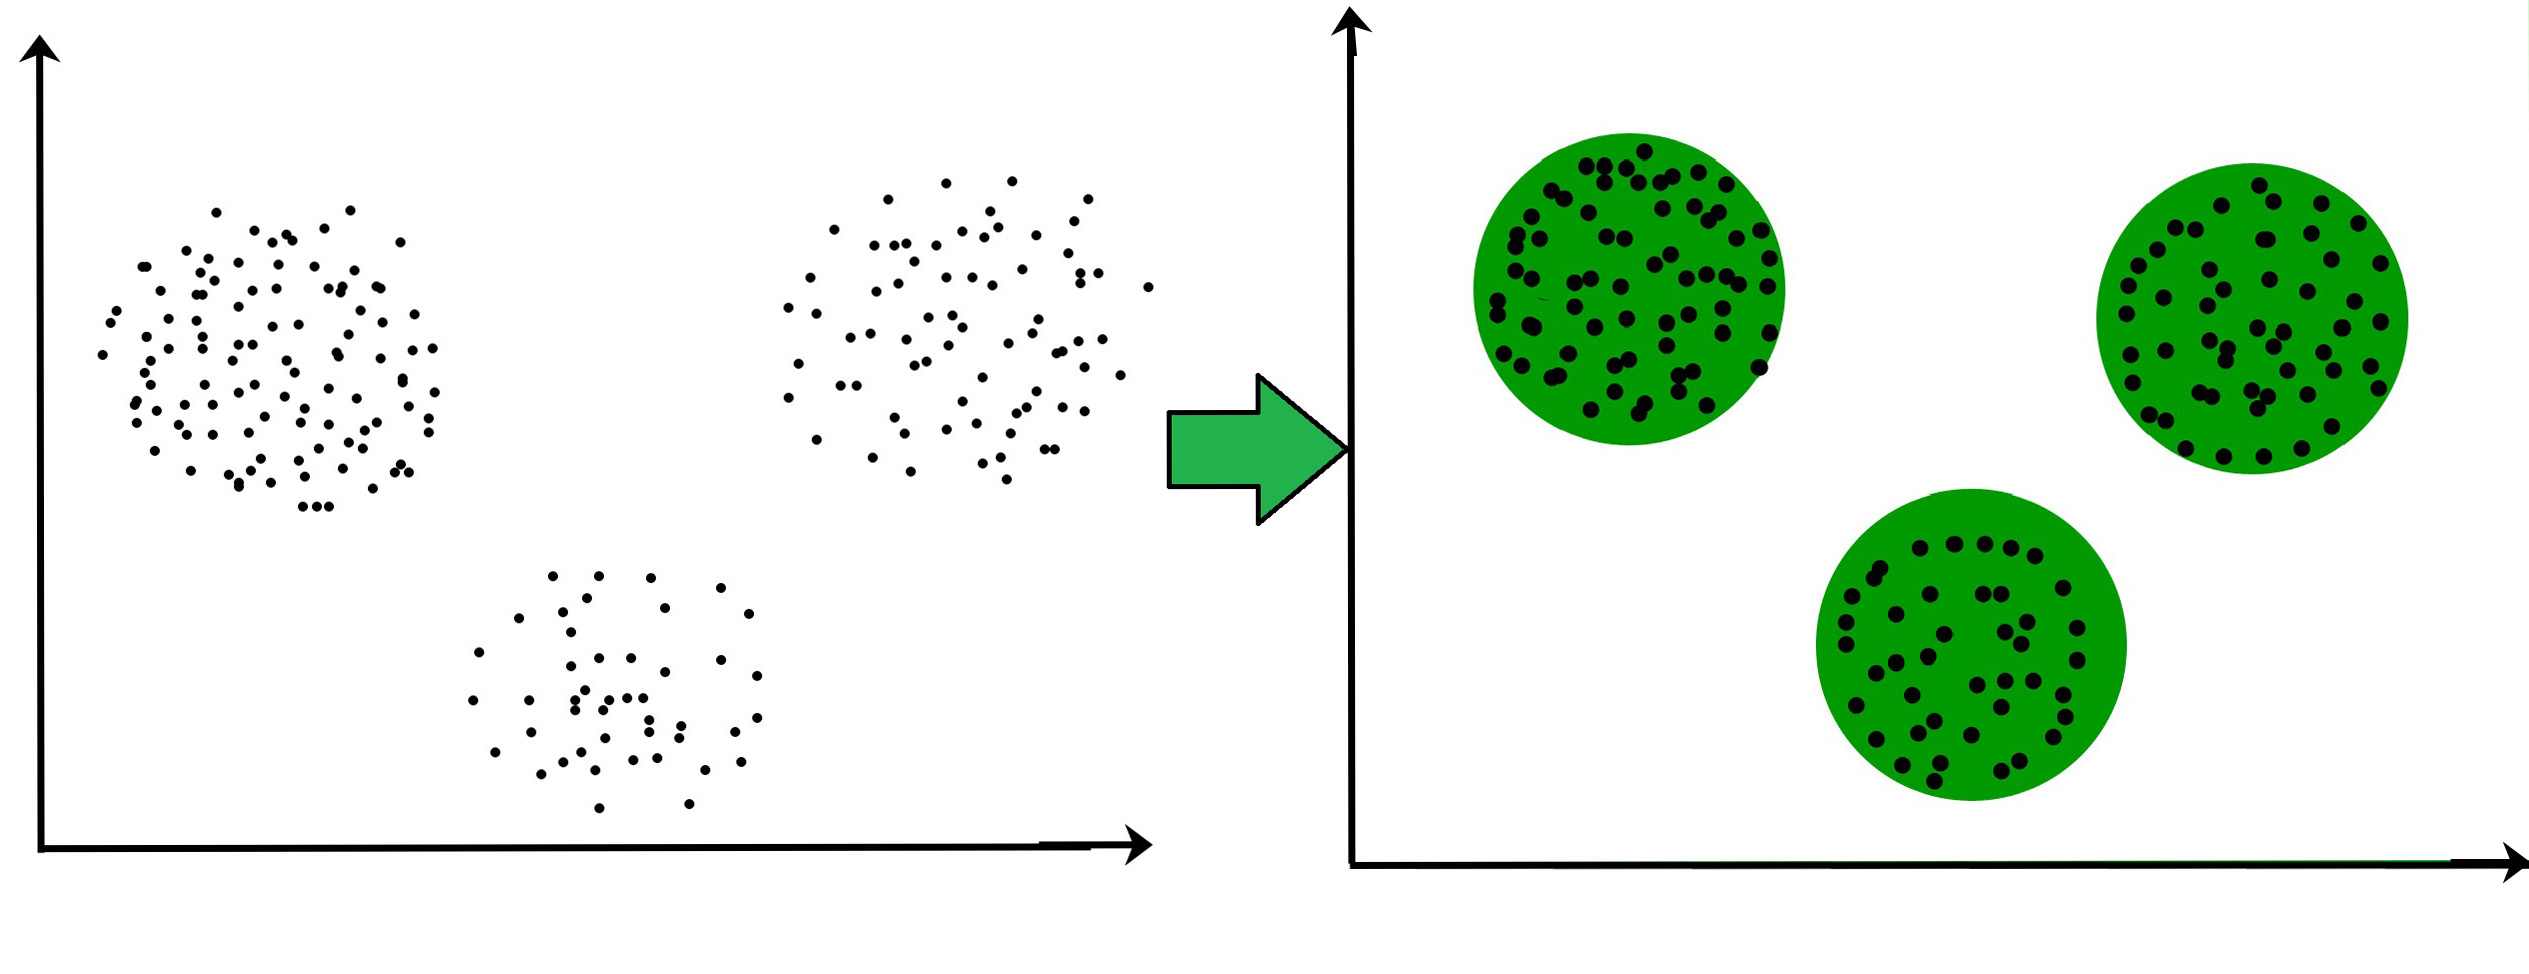
\includegraphics[width=\textwidth]{transformer_images/clustring.jpg}
		\caption{خوشه بندی}
		\label{fig:clustring}
	\end{minipage}
	\hfill
\end{figure}




\subsection{یادگیری تقویتی}
یادگیری تقویتی، \footnote{\lr{reinforcement learning}} نوعی یادگیری بر پایه پاداش و تنبیه است که در آن مدل با محیط تعامل می‌کند و بر اساس پاداش یا تنبیه یاد می‌گیرد
\cite{sutton2018reinforcement}.
برخلاف یادگیری نظارت‌شده و بدون نظارت، یادگیری تقویتی به مدل این امکان را می‌دهد تا از طریق آزمون و خطا بهترین راهکارها را برای انجام یک عمل یاد بگیرد. در این روش، مدل به جای برچسب، از یک تابع پاداش استفاده می‌کند که مشخص می‌کند چه اقداماتی باعث نتیجه بهینه می‌شود. از کاربردهای یادگیری تقویتی می‌توان به بازی‌ها \footnote{\lr{Games}}، کنترل رباتیک \footnote{\lr{Robotic Control}} و سیستم‌های توصیه‌گر \footnote{\lr{Recommender Systems}} اشاره کرد.



\begin{figure}[h]
	\centering
	\begin{minipage}[b]{0.8\textwidth}
		\centering
		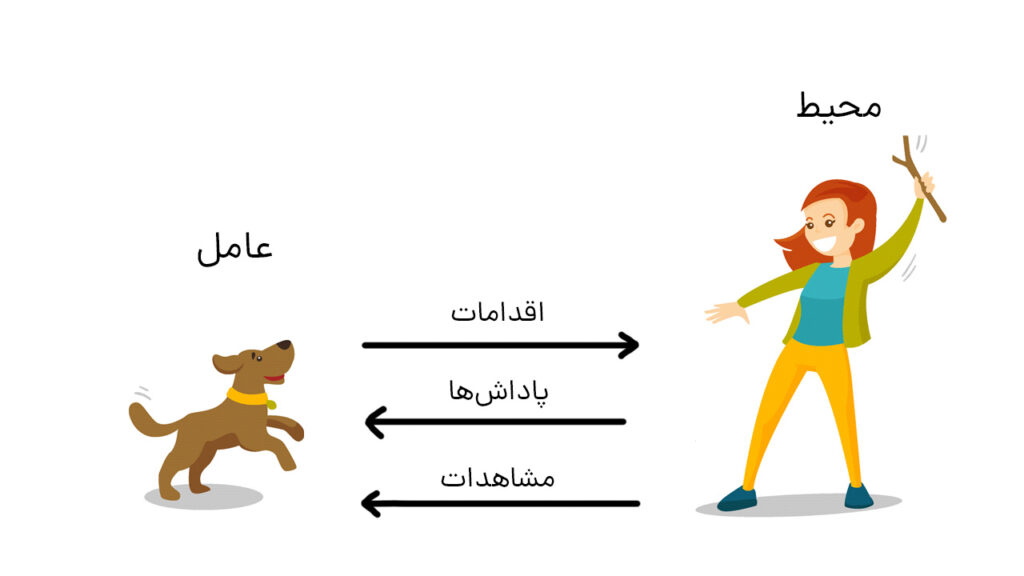
\includegraphics[width=\textwidth]{transformer_images/reinforcement_learning.jpg}
		\caption{یادگیری تقویتی}
		\label{fig:reinforcement learning}
	\end{minipage}
	\hfill
\end{figure}



\subsection{معرفی چند مدل از الگوریتم یادگیری کلاسیک}

الگوریتم‌های یادگیری کلاسیک، پایه و اساس بسیاری از پیشرفت‌های اولیه در یادگیری ماشین را شکل داده‌اند. این الگوریتم‌ها با وجود سادگی نسبی، در بسیاری از کاربردها همچنان عملکرد قابل قبولی از خود نشان می‌دهند و در بسیاری از سامانه‌های عملیاتی مورد استفاده قرار می‌گیرند.

الگوریتم‌هایی مانند نزدیک‌ترین همسایه \footnote{\lr{k-nearest neighbors algorithm
}}، ماشین بردار پشتیبان\footnote{\lr{Support vector machine
}}، بیز ساده\footnote{\lr{Naive Bayes}}و درخت تصمیم\footnote{\lr{Decision Tree}}از جمله مشهورترین روش‌های کلاسیک یادگیری هستند که هر یک بر اساس اصول ریاضی و آماری متفاوتی طراحی شده‌اند. این مدل‌ها معمولاً برای مسائل طبقه‌بندی یا رگرسیون به‌کار می‌روند و از مزایایی چون پیاده‌سازی آسان، قابلیت تفسیر بالا و نیاز کمتر به تنظیمات پیچیده برخوردارند.

در این بخش، به معرفی اجمالی چند مورد از این الگوریتم‌ها پرداخته می‌شود تا زمینه درک عمیق‌تر روش‌های نوین‌تر یادگیری، مانند شبکه‌های عصبی و مدل‌های عمیق، فراهم گردد.

\subsection{نزدیک‌ترین همسایه }

الگوریتم نزدیک‌ترین همسایه \footnote{\lr{k-Nearest Neighbors}} یکی از روش‌های ساده و درعین‌حال کارآمد در یادگیری نظارت‌شده است که هم در دسته‌بندی و هم در رگرسیون کاربرد دارد
\cite{cover1967nearest,duda1973pattern,mitchell1997machine}.
این الگوریتم برای پیش‌بینی دسته‌بندی یک نمونه جدید، به $k$ نزدیک‌ترین داده‌ها در فضای ویژگی نگاه می‌کند و بر اساس اکثریت نزدیکی همسایه‌ها، آن را به یک دسته اختصاص می‌دهد. 


\begin{figure}[h]
	\centering
	\begin{minipage}[b]{0.8\textwidth}
		\centering
		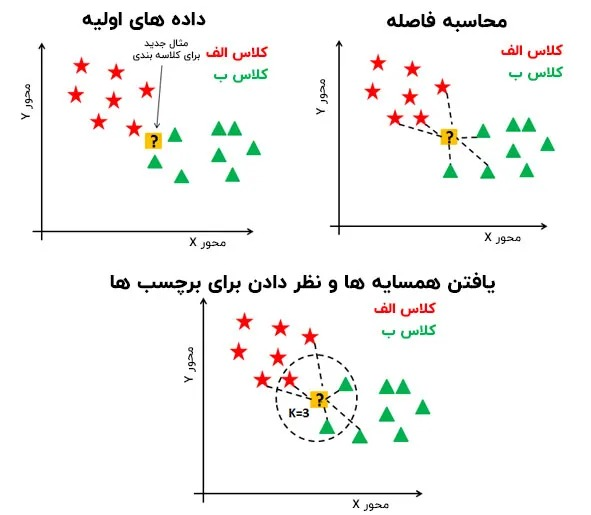
\includegraphics[width=\textwidth]{transformer_images/knn_11zon.jpg}
		\caption{الگوریتم نزدیکترین همسایه}
		\label{fig:k nearest neighbor}
	\end{minipage}
	\hfill
\end{figure}



از مهم‌ترین مزایای این الگوریتم می‌توان به \textbf{سادگی و قابل فهم بودن} اشاره کرد؛ چرا که تنها با اندازه‌گیری فاصله بین نقاط داده عمل می‌کند و بدون نیاز به آموزش یک مدل پیچیده، قابل استفاده است \cite{cover1967nearest}. همچنین، \textbf{عملکرد خوب در داده‌های با تعداد ویژگی کم} از دیگر نقاط قوت آن است، زیرا در مسائلی که تعداد ویژگی‌ها محدود است، این الگوریتم اغلب نتایج مطلوبی ارائه می‌دهد \cite{james2013introduction}.


در مقابل، الگوریتم نزدیک‌ترین همسایه دارای برخی معایب نیز هست. یکی از مهم‌ترین آن‌ها \textbf{حساسیت به داده‌های پرت} است؛ به‌طوری‌که نقاط پرت می‌توانند تأثیر قابل توجهی بر نتایج داشته باشند \cite{duda1973pattern}. علاوه بر این، \textbf{کندی در داده‌های بزرگ} از دیگر مشکلات این روش است، زیرا برای هر نقطه جدید نیاز به محاسبه فاصله با تمام داده‌ها دارد که در مجموعه‌داده‌های بزرگ منجر به بار محاسباتی بالا می‌شود \cite{mitchell1997machine}. در نهایت، این الگوریتم در \textbf{داده‌های با ابعاد بالا} کارایی مناسبی ندارد و با افزایش تعداد ویژگی‌ها عملکرد آن به طور محسوسی افت می‌کند \cite{murphy2012machine}.



\subsection{ماشین بردار پشتیبان}
الگوریتم ماشین بردار پشتیبان \footnote{\lr{Support Vector Machine, SVM}} با یافتن یک ابرصفحه بهینه، داده‌ها را به کلاس‌های مختلف تقسیم می‌کند
\cite{cortes1995support,vapnik1998statistical}.
این الگوریتم یک ابرصفحه به دست می‌آورد که هدف آن حداکثر کردن فاصله میان داده‌های دو کلاس است و به این ترتیب می‌تواند طبقه‌بندی دقیقی داشته باشد.

\begin{figure}[h]
	\centering
	\begin{minipage}[b]{0.8\textwidth}
		\centering
		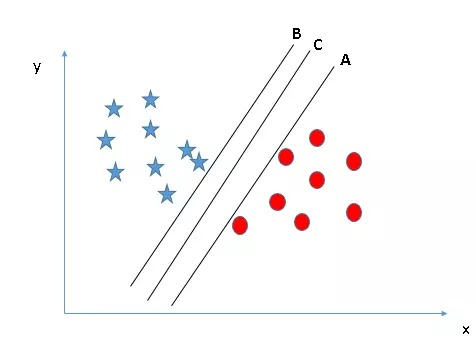
\includegraphics[width=\textwidth]{transformer_images/SVM_11zon.jpg}
		\caption{الگوریتم ماشین بردار پشتیبان}
		\label{fig:support vector machine}
	\end{minipage}
	\hfill
\end{figure}


از مهم‌ترین مزایای ماشین بردار پشتیبان می‌توان به \textbf{توانایی مقابله با داده‌های پیچیده و ابعاد بالا} اشاره کرد؛ این الگوریتم قادر است به خوبی داده‌های چندبعدی و پیچیده را مدیریت کند و در چنین شرایطی همچنان عملکرد دقیقی داشته باشد \cite{vapnik1998statistical}. علاوه بر این، \textbf{مقاومت در برابر بیش‌برازش \footnote{\lr{Overfitting}}} یکی دیگر از نقاط قوت آن است. با استفاده از توابع هسته \footnote{\lr{Kernels}}، داده‌های غیرخطی به فضای ویژگی‌های بالاتر نگاشت می‌شوند و این امکان فراهم می‌شود که مرز جداسازی بهتری میان کلاس‌ها ایجاد گردد \cite{cortes1995support}. 

با وجود مزایای ذکر شده، ماشین بردار پشتیبان معایبی نیز دارد. نخستین مسئله، \textbf{پیچیدگی محاسباتی} آن است؛ آموزش این الگوریتم به دلیل نیاز به حل مسائل بهینه‌سازی، در حجم‌های بالای داده بسیار زمان‌بر خواهد بود \cite{murphy2012machine}. همچنین، \textbf{کارایی پایین در داده‌های پرت} از دیگر نقاط ضعف آن است، چرا که وجود تعداد زیادی داده پرت می‌تواند به شکل قابل توجهی دقت مدل را کاهش دهد \cite{bishop2006pattern}.



\subsection{بیز ساده}
بیز ساده \footnote{Naive Bayes} مبتنی بر قضیه بیز \footnote{\lr{Bayes' theorem}}است و فرض می‌کند ویژگی‌ها به‌صورت شرطی مستقل از هم هستند\cite{domingos1997optimal,mitchell1997machine}.
این مدل برای اولین بار در حوزه پردازش متن به کار رفت و هنوز هم در بسیاری از کاربردها مانند طبقه‌بندی ایمیل و تحلیل احساسات مورد استفاده قرار می‌گیرد\cite{mccallum1998comparison}. 
در بیز ساده بر اساس احتمالات محاسبه می‌شود که یک نمونه جدید به کدام دسته تعلق دارد. این الگوریتم بر اساس قضیه بیز، احتمال تعلق یک نمونه به هر دسته را به ازای هر ویژگی محاسبه کرده و در نهایت بالاترین احتمال را به‌عنوان جواب نهایی در نظر می‌گیرد\cite{bishop2006pattern}.


از مهم‌ترین مزایای بیز ساده می‌توان به \textbf{سرعت بالا} اشاره کرد؛ چرا که به دلیل محاسبات ساده و فرض استقلال ویژگی‌ها، این الگوریتم بسیار سریع و کم‌حجم بوده و برای مسائل با داده‌های زیاد یا در شرایط نیاز به پاسخ بلادرنگ کارایی بالایی دارد \cite{mccallum1998comparison}. علاوه بر این، \textbf{کارایی در داده‌های کوچک} از دیگر نقاط قوت آن است، زیرا حتی با وجود حجم محدود داده‌ها، مدل همچنان قادر است عملکرد قابل قبولی ارائه دهد \cite{murphy2012machine}.  


با وجود مزایا، بیز ساده محدودیت‌هایی هم دارد. یکی از مهم‌ترین آن‌ها \textbf{فرض استقلال ویژگی‌ها}ست؛ فرضی که در بسیاری از مسائل واقعی برقرار نیست و می‌تواند باعث کاهش دقت مدل شود \cite{domingos1997optimal}. علاوه بر این، این الگوریتم نسبت به کیفیت داده‌ها بسیار حساس است و \textbf{حساسیت به داده‌های نادرست یا پرت} می‌تواند موجب کاهش چشمگیر دقت آن شود \cite{bishop2006pattern}.




\subsection{شبکه‌های عصبی بازگشتی و شبکه‌های حافظه بلندمدت کوتاه‌مدت}
شبکه‌های عصبی بازگشتی \footnote{\lr{RNN}} و مدل‌هایی با حافظهٔ بلندمدت-کوتاه‌مدت \footnote{\lr{LSTM}} با هدف پردازش داده‌های ترتیبی و وابسته به زمان توسعه یافتند
\cite{rumelhart1986learning,hochreiter1997long}.
این مدل‌ها به‌ویژه در تحلیل زبان طبیعی، پردازش صوت و پیش‌بینی سری‌های زمانی بسیار موفق عمل کرده‌اند؛ زیرا قادر به حفظ اطلاعات گذشته هستند و از این اطلاعات برای پیش‌بینی در لحظهٔ حال و آینده استفاده می‌کنند
\cite{gers1999learning}.

\subsection{شبکه‌های عصبی بازگشتی}
مدل‌های اولیه شبکه‌های عصبی، مانند شبکه‌های چندلایه \footnote{\lr{MLP}}، قادر به پردازش داده‌های مستقل و ثابت بودند و نمی‌توانستند وابستگی‌های زمانی را یاد بگیرند\cite{bishop2006pattern}.
در بسیاری از مباحث دنیای واقعی مانند تحلیل متن، صدا و  داده‌ها به توالی خاصی وابسته هستند. به همین دلیل، شبکه‌های عصبی بازگشتی معرفی شدند تا بتوانند از اطلاعات پیشین در پردازش داده‌های بعدی استفاده کنند\cite{rumelhart1986learning}.


\subsection{ساختار و عملکرد شبکه‌های عصبی بازگشتی}
شبکه‌های عصبی بازگشتی \footnote{\lr{Recurrent Neural Network}} دارای حلقه بازگشتی هستند که به مدل این امکان را می‌دهد اطلاعات را در توالی نگه دارد و در هر گام زمانی، ورودی فعلی \( x_t \) و وضعیت قبلی \( h_{t-1} \) را به‌عنوان ورودی دریافت کند \cite{goodfellow2016deep}.  

\begin{figure}[h]
	\centering
	\begin{minipage}[b]{0.7\textwidth}
		\centering
		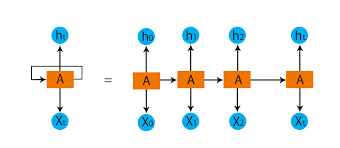
\includegraphics[width=\textwidth]{transformer_images/rnn_image.png}
		\caption{شبکه‌های عصبی بازگشتی}
		\label{fig:recurrent neural network}
	\end{minipage}
	\hfill
\end{figure}

\begin{equation}
	h_t = \sigma \big( W \cdot x_t + U \cdot h_{t-1} + b \big)
\end{equation}

در این رابطه، \( h_t \) نشان‌دهنده وضعیت مخفی یا حالت در گام زمانی \( t \) است. ماتریس \( W \) وزن‌هایی را مشخص می‌کند که به ورودی \( x_t \) اعمال می‌شوند، در حالی که ماتریس \( U \) وزن‌های مربوط به وضعیت قبلی \( h_{t-1} \) را در نظر می‌گیرد. مقدار \( b \) بایاس مدل است و در نهایت، تابع \(\sigma\) نقش تابع فعال‌سازی را ایفا می‌کند که معمولاً از نوع تانژانت هیپربولیک یا سیگموید انتخاب می‌شود. به کمک این ساختار، مدل می‌تواند اطلاعات گذشته را در خود ذخیره کرده و در پردازش‌های بعدی از آن‌ها بهره ببرد.  


از مهم‌ترین مزایای شبکه‌های عصبی بازگشتی می‌توان به \textbf{حفظ وابستگی زمانی} اشاره کرد. این مدل‌ها قادر به پردازش توالی‌های طولانی هستند و می‌توانند اطلاعات پیشین را در طول توالی به خاطر بسپارند و در تصمیم‌گیری‌های بعدی به کار گیرند \cite{elman1990finding}. همچنین، \textbf{کاربردهای گسترده در داده‌های ترتیبی} از دیگر نقاط قوت آن‌هاست؛ چرا که در حوزه‌هایی مانند تحلیل زبان طبیعی، پیش‌بینی سری‌های زمانی و پردازش صوت، نتایج بسیار موفقی داشته‌اند \cite{gers1999learning}.  

با وجود این مزایا، شبکه‌های عصبی بازگشتی معایبی هم دارند. یکی از اصلی‌ترین مشکلات آن‌ها \textbf{ناپدید شدن و انفجار گرادیان \footnote{\lr{Vanishing and Exploding Gradient}}} است. در فرایند آموزش با روش پس‌انتشار \footnote{\lr{Backpropagation}}، اگر توالی داده‌ها طولانی باشد، گرادیان‌ها ممکن است بسیار کوچک یا بسیار بزرگ شوند که این امر منجر به ناپایداری در آموزش و کاهش دقت می‌شود \cite{hochreiter1998vanishing}. علاوه بر این، این شبکه‌ها \textbf{محدودیت در پردازش توالی‌های بسیار بلند} دارند؛ به این معنا که در حفظ وابستگی‌های طولانی‌مدت دچار مشکل شده و عملکرد ضعیفی نشان می‌دهند \cite{hochreiter1997long,goodfellow2016deep}.

\subsection{شبکه‌های حافظه بلندمدت-کوتاه‌مدت}

شبکه‌های حافظه بلندمدت-کوتاه‌مدت به عنوان یک راه‌حل برای یکی از بزرگ‌ترین مشکلات شبکه‌های عصبی بازگشتی معرفی شدند
\cite{hochreiter1997long}.
یکی از برجسته‌ترین مشکلات موجود در شبکه‌های عصبی بازگشتی، معضل ناپدید شدن گرادیان  بود که مانع یادگیری وابستگی‌های بلندمدت می‌شد
\cite{hochreiter1998vanishing,goodfellow2016deep}.
برای درک عمیق‌تر این مسأله، ابتدا به توضیح مشکل ناپدید شدن گرادیان و سپس راهکار شبکه‌های حافظه بلندمدت-کوتاه‌مدت می‌پردازیم.

\subsection{ناپدید شدن گرادیان در شبکه های بازگشتی}
شبکه‌های عصبی بازگشتی برای پردازش داده‌های ترتیبی از حلقه‌های بازگشتی بهره می‌برند. در فرایند آموزش شبکه‌های عصبی بازگشتی، از الگوریتم پس‌انتشار خطا از طریق زمان \footnote{\lr{Backpropagation Through Time}} استفاده می‌شود که گرادیان‌ها را جهت به‌روزرسانی وزن‌ها محاسبه می‌کند.\cite{rumelhart1986learning}.

با این حال، شبکه های عصبی بازگشتی در یادگیری وابستگی‌های بلندمدت معمولاً ناکام می‌مانند. علت اصلی این امر شامل موارد زیر است:

\begin{itemize}
	\item \textbf{ضریب‌های بازگشتی کوچک‌تر از ۱:}
	در فرایند محاسبهٔ گرادیان‌ها، اگر مقدار مشتقات یا ضرایب در هر مرحله کوچک‌تر از ۱ باشد، ضرب مکرر این ضرایب در طول توالی منجر به کوچک‌شدن گرادیان‌ها به سمت صفر می‌شود؛ پدیده‌ای که به ناپدید شدن گرادیان\footnote{\lr{vanishing gradient}} معروف است
	\cite{hochreiter1998vanishing}.
\end{itemize}

فرمول کلی گرادیان در زمان \( t \) به‌صورت زیر است:

\begin{equation}
	\frac{\partial L}{\partial W} = \prod_{k=1}^{t} \frac{\partial h_k}{\partial h_{k-1}} \cdot \frac{\partial h_t}{\partial L}
\end{equation}

در این فرمول، \( \frac{\partial h_k}{\partial h_{k-1}} \) ممکن است مقداری کوچک‌تر از ۱ باشد، و ضرب مکرر آن در طول توالی باعث کاهش شدید مقدار گرادیان می‌گردد.

\begin{itemize}
	\item \textbf{تأثیر مستقیم بر وزن‌ها:}
	زمانی که گرادیان‌ها به صفر نزدیک می‌شوند، وزن‌های مدل عملاً به‌روزرسانی نمی‌شوند و این امر مانع از یادگیری وابستگی‌های طولانی‌مدت در داده‌ها می‌شود\cite{goodfellow2016deep}.
\end{itemize}

\subsection{ظهور شبکه‌های حافظه بلندمدت-کوتاه‌مدت}
در سال ۱۹۹۷،شبکه‌های حافظه بلندمدت-کوتاه‌مدت  معرفی شد.
\cite{hochreiter1997long}.
انگیزه اصلی توسعه این شبکه حل مشکل ناپدید شدن گرادیان در شبکه‌های عصبی بازگشتی بود. این مشکل در مسائل یادگیری داده‌های ترتیبی طولانی مانع می‌شد شبکه های عصبی بازگشتی وابستگی‌های بلندمدت را به‌درستی فراگیرد.

\subsection{راه‌حل شبکه‌های حافظه بلندمدت-کوتاه‌مدت برای پایداری جریان گرادیان‌ها}
 با معرفی شبکه حافظه بلند مدت، کوتاه مدت \footnote{\lr{long short-term memory}} در شبکه‌های بازگشتی، جریان گرادیان‌ها را در طول توالی پایدار نگه می‌دارد. این کار از طریق اضافه کردن وضعیت سلولی \footnote{\lr{Cell State}} و دروازه‌ها \footnote{\lr{Gates}} به ساختار شبکه‌های عصبی بازگشتی انجام می‌شود.
\cite{gers1999learning}.
این اجزا به این شبکه این امکان را می‌دهند:

\begin{enumerate}
	\item اطلاعات غیرضروری را فراموش کند،
	\item اطلاعات مهم جدید را اضافه کند،
	\item اطلاعات مهم قبلی را حفظ کند.
\end{enumerate}

\section{ساختار شبکه های حافظه بلند-مدت کوتاه-مدت}
شبکه های حافظه بلند-مدت  شامل اجزای جدیدی است که به آن امکان مدیریت بهتر اطلاعات را می‌دهد:




\subsection{وضعیت سلولی}
مسیر اصلی ذخیره اطلاعات در  شبکه های حافظه بلند-مدت کوتاه مدت است که می‌تواند اطلاعات مهم را در طول توالی حفظ کند. برخلاف شبکه های عصبی بازگشتی که عمدتاً بر خروجی‌های بازگشتی \( h_t \) متکی است،  شبکه حافظه بلند مدت، کوتاه مدت  یک مسیر جداگانه برای عبور اطلاعات از وضعیت سلولی دارد که به حفظ گرادیان‌ها کمک شایانی می‌کند
\cite{hochreiter1997long}.


 \begin{figure}[h]
	\centering
	\begin{minipage}[b]{0.7\textwidth}
		\centering
		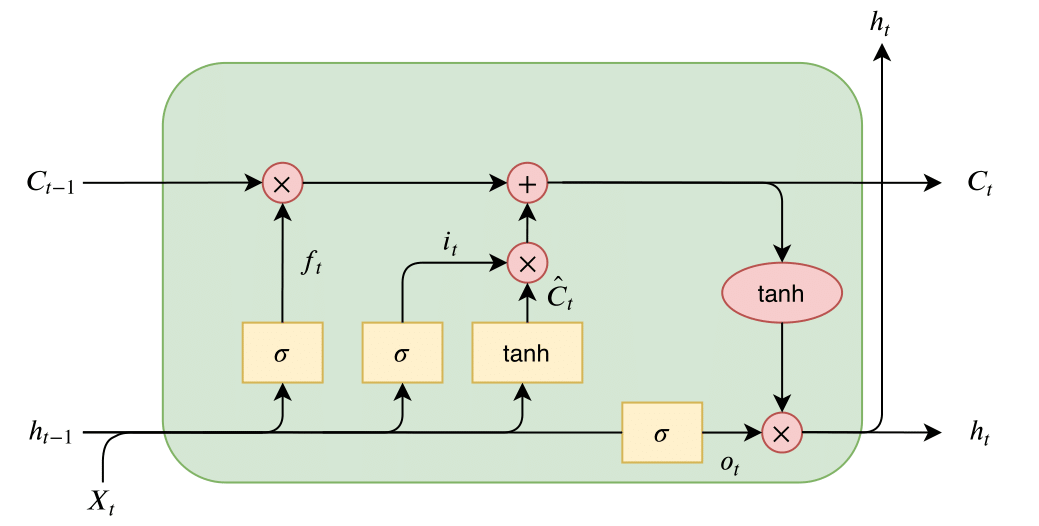
\includegraphics[width=\textwidth]{transformer_images/lstm.png}
		\caption{مدل حافظه بلند مدت کوتاه مدت}
		\label{fig:LSTM}
	\end{minipage}
	\hfill
	
\end{figure}


\subsection{دروازه‌ها}
دروازه‌ها نقش فیلترهای اطلاعاتی را دارند که جریان اطلاعات را در طول فرایند یادگیری کنترل می‌کنند.


    \textbf{دروازه فراموشی \footnote{\lr{Forget Gate}}}
	تعیین می‌کند چه اطلاعاتی از وضعیت سلولی باید حذف شود
	\cite{gers1999learning}.
	
	\begin{equation}
		f_t = \sigma \big( W_f \cdot [h_{t-1}, x_t] + b_f \big)
	\end{equation}

در این معادله، \( f_t \) بیانگر میزان فراموشی برای هر مؤلفه از وضعیت سلولی در گام زمانی جاری است. این مقدار با استفاده از تابع فعال‌ساز سیگموید \( \sigma \) محاسبه می‌شود که خروجی آن بین صفر تا یک قرار دارد. هرچه مقدار \( f_t \) به صفر نزدیک‌تر باشد، آن مؤلفه از وضعیت سلولی بیشتر فراموش می‌شود؛ و بالعکس، مقدار نزدیک به یک نشان‌دهنده حفظ کامل آن اطلاعات در حافظه سلولی است.



	\textbf{دروازه ورودی \footnote{\lr{Input Gate}}:}
	تعیین می‌کند چه اطلاعات جدیدی باید به وضعیت سلولی اضافه شود:
	\begin{equation}
		i_t = \sigma \big( W_i \cdot [h_{t-1}, x_t] + b_i \big)
	\end{equation}
	
	\begin{equation}
		\tilde{C}_t = \tanh \big( W_C \cdot [h_{t-1}, x_t] + b_C \big)
	\end{equation}

	که در آن \( i_t \) میزان اطلاعات جدید و \( \tilde{C}_t \) مقدار جدید قابل اضافه‌شدن به وضعیت سلولی را نشان می‌دهد.
	
\textbf{دروازهٔ خروجی \footnote{\lr{Output Gate}}:}

	تعیین می‌کند چه اطلاعاتی از وضعیت سلولی به خروجی منتقل شود:
	\[
	o_t = \sigma \big( W_o \cdot [h_{t-1}, x_t] + b_o \big),
	\]
	\[
	h_t = o_t \cdot \tanh(C_t).
	\]


\subsection{به‌روزرسانی وضعیت سلولی}
وضعیت سلولی \( C_t \) با استفاده از اطلاعات جدید و قدیمی به‌روزرسانی می‌شود:
	\begin{equation}
		C_t = f_t \cdot C_{t-1} + i_t \cdot \tilde{C}_t
	\end{equation}

این ساختار باعث می‌شود اطلاعات قدیمی مهم حفظ و داده‌های غیرضروری حذف شوند.

\subsubsection{ علت پایداری گرادیان در شبکه های حافظه بلند-مدت کوتاه مدت}
\begin{itemize}
	\item \textbf{حذف ضرب‌های مکرر:}
	برخلاف شبکه های بازگشتی که به ضرب‌های مکرر وزن‌ها و گرادیان‌ها وابسته است، شبکه های حافظه بلند-مدت کوتاه مدت با مسیر جداگانهٔ وضعیت سلولی، از کاهش نمایی گرادیان جلوگیری می‌کند
	\cite{hochreiter1998vanishing}.
	
	\item \textbf{استفاده از توابع سیگموید و تانژانت هیپربولیک:}
	توابع سیگموید در دروازه‌ها و تانژانت هیپربولیک در وضعیت سلولی مقادیر را محدود می‌کنند و مانع از انفجار گرادیان می‌شوند\cite{gers1999learning,goodfellow2016deep}.
	
	\item \textbf{مدیریت اطلاعات توسط دروازه‌ها:}
	دروازه‌های فراموشی و ورودی به مدل اجازه می‌دهند تنها اطلاعات مهم حفظ شود و داده‌های غیرضروری حذف شوند.این موضوع از پیچیدگی محاسباتی غیرضروری جلوگیری می‌کند
	\cite{hochreiter1997long}.
\end{itemize}

\begin{table}[h!]
	\centering
	\resizebox{\columnwidth}{!}{%
		\begin{tabular}{|c|c|c|}
			\hline
			\textbf{ویژگی} & \textbf{RNN} & \textbf{LSTM} \\ \hline
			\textbf{مشکل ناپدید شدن گرادیان} & وجود دارد & برطرف شده \\ \hline
			\textbf{توانایی حفظ وابستگی‌های طولانی‌مدت} & محدود به وابستگی کوتاه‌مدت & بسیار خوب \\ \hline
			\textbf{ساختار دروازه‌ها} & ندارد & دارای دروازه‌های فراموشی، ورودی و خروجی \\ \hline
			\textbf{پایداری گرادیان} & ضعیف & پایدار \\ \hline
		\end{tabular}%
	}
	\caption{مقایسه ویژگی‌های RNN و LSTM}
\end{table}



\subsection{محدودیت‌های شبکه‌های بازگشتی}
شبکه‌های بازگشتی داده‌ها را به‌صورت ترتیبی پردازش می‌کنند؛ به این معنی که برای پردازش داده‌های گام زمانی \( t \)، باید تمامی داده‌های قبلی (\( t-1 \)) پردازش شده باشند \cite{rumelhart1986learning,hochreiter1997long}. این ویژگی موجب می‌شود که پردازش داده‌ها به صورت موازی امکان‌پذیر نباشد و همین امر زمان محاسباتی را افزایش دهد. در داده‌های بلند، مانند متن‌های طولانی یا سری‌های زمانی بزرگ، این مشکل نمود بیشتری پیدا می‌کند. علاوه بر این، پردازش خطی داده‌ها موجب کندی در آموزش و استنتاج مدل‌ها می‌شود، به‌ویژه زمانی که حجم داده‌ها بسیار زیاد باشد.  

با وجود پیشرفت‌هایی که در شبکه‌های حافظه بلندمدت-کوتاه‌مدت نسبت به شبکه‌های بازگشتی معمولی حاصل شده است، این مدل‌ها همچنان در یادگیری وابستگی‌های بسیار طولانی محدودیت دارند \cite{hochreiter1998vanishing}. به طور مثال، در جملات طولانی ممکن است ارتباط میان کلمات ابتدایی و انتهایی اهمیت بالایی داشته باشد، اما ظرفیت این شبکه‌ها در حفظ چنین اطلاعاتی محدود است و با افزایش طول توالی، دقت مدل کاهش می‌یابد. همچنین داده‌های ابتدایی توالی به مرور اهمیت خود را از دست می‌دهند، زیرا گرادیان‌ها به تدریج ضعیف‌تر می‌شوند.  

از سوی دیگر، ساختار پیچیده شبکه‌های حافظه بلندمدت-کوتاه‌مدت، که شامل چندین ماتریس ضرب برای دروازه‌های ورودی، خروجی و فراموشی و به‌روزرسانی وضعیت سلول است، باعث افزایش نیاز به حافظه و محاسبات می‌شود \cite{goodfellow2016deep}. در مقیاس‌های بزرگ، این موضوع به افزایش هزینهٔ محاسباتی و کندی اجرای مدل منجر می‌گردد.  

شبکه‌های بازگشتی همچنین در پردازش وابستگی‌های غیرمتوالی با محدودیت‌هایی روبه‌رو هستند. برای مثال، در ترجمه زبان یا تحلیل متون طولانی، ممکن است کلمه‌ای در ابتدای جمله با کلمه‌ای در انتهای آن ارتباط معنایی داشته باشد \cite{bahdanau2014neural}. این نوع وابستگی‌های غیرمحلی برای شبکه‌های بازگشتی به سختی قابل یادگیری است.  

مشکل دیگر به پایداری گرادیان‌ها بازمی‌گردد. با وجود بهبودهایی که شبکه‌های حافظه بلندمدت-کوتاه‌مدت در این زمینه نسبت به شبکه‌های بازگشتی معمولی داشته‌اند، همچنان در توالی‌های بسیار بلند گرادیان‌ها ممکن است دچار کاهش یا انفجار شوند که این مسئله پایداری آموزش و دقت مدل را تحت تأثیر قرار می‌دهد \cite{hochreiter1998vanishing}. افزون بر این، در مسائل پیچیده یافتن مینیمم مناسب تابع هزینه دشوار است و بهینه‌سازی مدل با چالش روبه‌رو می‌شود.  

در نهایت، شبکه‌های بازگشتی برای مسائل پیچیده‌تر به ظرفیت و سرعت بالاتری نیاز دارند، اما محدودیت در حافظه و پردازش مانع از دستیابی به این هدف می‌شود. همچنین این مدل‌ها در داده‌های چندوجهی \footnote{\lr{Multimodal}}، مانند داده‌هایی که ترکیبی از متن، صوت و تصویر هستند، عملکرد مناسبی ندارند؛ زیرا توانایی لازم برای پردازش موازی این نوع اطلاعات را در اختیار ندارند.

در مجموع، وابستگی ترتیبی در شبکه های بازگشتی مانعی اساسی برای استفاده از این مدل‌ها در مسائل پیچیده و بزرگ بود که درنهایت به ظهور مبدل ها منتهی شد
\cite{vaswani2017attention}.
مبدل‌ها با طراحی مبتنی بر موازی‌سازی و مکانیزم توجه \footnote{\lr{Attention Mechanism}}، این محدودیت را برطرف کرده و راه‌حلی کارآمدتر برای پردازش داده‌های ترتیبی ارائه دادند.




